%! TEX root = ../main.tex
\chapter{Propuesta de solución}
\label{chap:solucion}


\observacion{\textbf{Mirti}:
\begin{itemize}
\item Estructurar de nuevo el capítulo de solución 
\item Que se quiere hacer,
    que hay para hacer (herramientas), la solución en sí (más gráficos que
    explicaciones)
\item Grafo de dependencia de pasos (requisitos)
\item Disminuir texto
\item Elementos -> partes -> específico esc1 -> específico esc 2
    \item Imágenes con indicaciones
\item Que información se puede sacar de los logs
\item Poner por partes la conclusión
\item motor gráfico no es lo mismo motor de juegos
\item Punto medio para descripción de los motores (definir los criterios que
    todos deben tener)
\item Ver formato de la tabla comparativa
\end{itemize}
}

\observacion{Arturo:
\begin{itemize}
\item Decir que se quiere usar tecnologías móviles
\item Grafo de dependencias
\item No describir lo que se podría mostrar con una imagen
\item Mencionar partes del motor de videojuegos
\item Nuevo orden de caps:
    \begin{enumerate}
    \item Problema
    \item Requisitos o descripción (incluir retroalmientación)
        \begin{itemize}
        \item Que se quiere hacer
        \item Grafo de pasos
        \end{itemize}
    \item Motores y tecnologías
        \begin{itemize}
        \item motores (Descripción y comparación)
        \item Simulación (entidades, etc)
        \end{itemize}
    \item Solución
\end{enumerate}
\item Presentar para el lunes
    \begin{itemize}
        \item Introducción
        \item TICS
        \item Formato de impresión (a la derecha)
        \item Un capítulo siempre empieza en la página impar
    \end{itemize}
\end{itemize}}

\fixme{En el capitulo anterior, se describieron los fundamentos teóricos del uso de
    videojuegos serios en el ambiente educativo, dicha descripción se centra en
    aquellas áreas que requieren más practica para la adquisición de la pericia
    necesaria. Así, se identifico el área de enfermería como problemática, la
    formación de enfermeros y se selecciona algunos procedimientos que serán
    utilizados para el contenido de la solución}{}. A continuación se busca converger
todos los aspectos descriptos en capítulos anteriores.

La solución propuesta en este trabajo consiste en el desarrollo de una
aplicación para dispositivos móviles que se define como un juego serio llamado
\fixme{\Gls{yave}}{No es tarde para cambiar de nombre!}, basado en el
\fixme{construccionismo}{?}, el cual incluye conceptos de la gamificación, y de
simulación. El juego consiste en ofrecer a los usuarios, en este caso alumnos de
enfermería, un medio en el cual puedan realizar procedimientos de enfermería y
cuyo objetivo es servir como herramienta de apoyo en el aprendizaje.

\Gls{yave} permite al usuario poder seleccionar el procedimiento que quiera
realizar, dando la posibilidad de interactuar con un paciente y con una conjunto
de objetos que forman parte de las herramientas requeridas para realizar el
procedimiento seleccionado. Además, contempla la posibilidad de realizar
acciones relacionadas a la bioseguridad, y otros aspectos transversales a la
educación de un enfermero.

La solución no solo le permite al usuario realizar los procedimientos para
poner en practica sus conocimientos sobre el mismo, sino también evaluará al
usuario, dándole al final de cada sesión una puntuación y describiendo los
pasos realizados correcta e incorrectamente, proporcionando información acerca
de los puntos incorrectos.

%! TEX root = ../main.tex

\section{Arquitectura general}
\label{sec:solucion}

\observacion{Siempre ayuda poner alguna imagen}
\observacion{Tunear esta intro}

A continuación se describe la arquitectura propuesta para la realización de una
juego serio, se utiliza la guía básica definida por~\cite{pereira2009design} y
descrita en~\ref{sec:desarrollo}.

Esta sección se enfoca en los aspectos técnicos de la creación del juego serio,
las competencias básicas relacionadas con la educación (segundo paso de la guía
descrita en~\ref{sec:desarrollo}) se definieron en las
secciones~\ref{sec:glasgow} y~\ref{sec:hemocultivo}.

\subsection{Grafo de estados}
\observacion{De? Grafo de estado de qué?}

\observacion{
\begin{itemize}
    \item Problema + escena
    \item Solución + descripción de escenas simuladas
    \item Tecnologías
    \item Implementación de escenas
\end{itemize}
}

La solución tiene varios escenarios, y dentro de cada escenario, existen varias
pantallas que muestran información relevante de acuerdo a la situación de la
simulación, en~\ref{fig:grafo_estados} se observa la interacción entre las
diferentes pantallas y escenarios.

\begin{figure}[H] 
\centering 
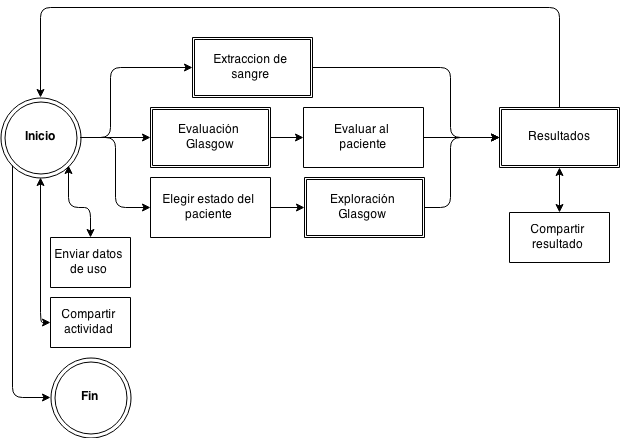
\includegraphics[scale=0.5]{propuesta/images/grafo_escenas.png}
\caption{Navegación entre escenarios y pantallas. Los escenarios son los
    rectángulos con un borde de dos rayas, y las pantallas tienen un borde con una
    sola raya. Los estados inicial y final se muestran como círculos, notar que
    el estado inicial es además del punto de entrada, un escenario.}
\label{fig:grafo_estados}
\end{figure}

La solución inicia con un escenario denominado \emph{Inicio}, en el cual se
permite al usuario observar los detalles del entorno simulado a la vez que
muestra las opciones que permiten iniciar las diferentes prácticas, compartir
su actividad, enviar los datos de utilización y finalmente salir de la
simulación.

Si el usuario selecciona en el \emph{inicio} la opción \emph{Extracción de
    sangre}, se inicia el escenario denominado \emph{Extracción de sangre}, en
el cual el usuario puede realizar el procedimiento de extracción de sangre, si
el usuario selecciona la opción \emph{Fin}, la simulación termina y se dirige 
al escenario \emph{Pantalla de resultados}.

Al seleccionar la opción \emph{Evaluación Glasgow}, se inicia el escenario
denominado \emph{Glasgow}, donde el usuario debe evaluar a un paciente en el
centro del escenario, si el usuario presiona la opción \emph{Fin} se inicia la
pantalla denominada \emph{Evaluar al paciente}, donde el usuario diagnostica el
estado del paciente, y finalmente al presionar el botón \emph{Fin}, la
simulación finaliza y se inicia el escenario \emph{Pantalla de resultados}.

La opción \emph{Exploración Glasgow} es similar, la diferencia es que antes de
iniciar el escenario \emph{Glasgow}, aparece la pantalla \emph{Elegir estado de
    paciente}, en el cual el usuario selecciona un estado para que el paciente
actué de acuerdo al mismo, luego se inicia la escena \emph{Glasgow} y si el
usuario presiona el botón \emph{Fin}, se inicia el escenario \emph{Pantalla de
    resultados}.

La pantalla de resultados muestra la información acerca de las acciones que
realizó el usuario, proveyendo información a modo de retroalimentación, en esta
pantalla el usuario puede compartir sus resultados por las redes sociales,
reiniciar el escenario y finalmente, puede volver a la \emph{Pantalla de
    inicio}.

A continuación, se describen todos los escenarios, primeramente se da una 
descripción general de los escenarios y se procede a explicar los detalles 
de los mismos, incluyendo las entidades, eventos y acciones que pueden ser realizados 
en el mismo.

\observacion{Se tiene que poder explicar esto sin ser tan verboso}

\subsection{Partes de la simulación}

La simulación se compone de tres elementos principales, entidades (que son
objetos de la vida real), acciones (que son provocadas por las entidades) y
eventos (que son el resultado de una acción). 

Existen otros elementos dentro de la simulación, como la sala y la iluminación,
los mismos son importantes para crear un entorno similar a la realidad y son
estáticos, es decir no interactúan con el usuario más que para limitar la
exploración en el escenario y/o resaltar aspectos relevantes.

\subsubsection{Entidades}

Una entidad es cualquier objeto o componente en el sistema que requiera la representación
explícita en el modelo\cite{banks2000dm}. Las entidades tienen atributos. Los
atributos son las características de una determinada entidad que son exclusivos
de esa entidad.

Una entidad tiene en todo momento, un estado y una lista de acciones que
puede realizar, esta lista de acciones esta definida por el estado del mismo,
las condiciones en la que se encuentra el entorno y la práctica actual.

La entidad \enquote{Enfermero} es la que es controlada por el usuario, a través
de la interacción con la interfaz gráfica.

\subsubsection{Acciones}

Las entidades se comunican a través de acciones, las cuales pueden tener
diversos orígenes, siempre una entidad inicia una acción. Las acciones provocan
cambios en el ambiente y provocan eventos. Las acciones no solo las
realiza el usuario, sino cualquier entidad.

Como ejemplo, una acción es esterilizar las manos, esta acción provoca un
cambio en el ambiente (las manos ahora son estériles) y fue realizada por la
interacción entre el usuario y la interfaz gráfica.

\subsubsection{Eventos}

Los eventos son ocurrencias instantáneas que cambian el estado de un
sistema\cite{banks2000dm}, cada acción que se realiza provoca otra acción, y los
eventos son el mecanismo que tiene una entidad para ser notificada de las
acciones de otras entidades.

Un evento es una consecuencia de una acción, por ejemplo, cuando el usuario 
realiza la acción \emph{Limpiar manos}, se crea el evento \emph{Manos Limpias}. 
Cualquier entidad de la simulación puede reaccionar ante diversos eventos, 
por ejemplo, la entidad \emph{Enfermero} reacciona ante el evento \emph{Manos
Limpias}, y cambia su estado interno para reflejar este evento (de ahora en 
más, se considera que las manos del enfermero están limpias).

Los Eventos son útiles para que varias entidades puedan reaccionar ante
una acción, cuando el enfermero extrae la jeringa del paciente, se crea un
evento para notificar este cambio, y el paciente reacciona de diversas maneras,
por ejemplo, desde ese momento, la zona de donde se extrajo la jeringa, pasa a 
estar contaminada. 

Existe otro componente además de las entidades que depende de los eventos 
para cambiar su estado, y es el \emph{Motor de Reglas}, este motor escucha
todos los eventos relacionados con las reglas, y se encarga de evaluar, así
es notificado de los cambios en el entorno.

\subsubsection{Interacción la escena}

El usuario se desenvuelve en un entorno de tres dimensiones, en el cual realiza las
actividades relacionadas a la práctica, se distinguen dos tipos de movimientos
principales que el usuario puede realizar:

\begin{itemize}
    \item \textbf{Alejamiento o acercamiento}: es el acto de acercar o alejar la
        cámara, y por consiguiente al usuario del paciente. Se realiza
        utilizando dos dedos, para realizar un acercamiento, mientras se
        mantiene presionada la pantalla con ambos dedos, se procede a alejar un
        dedo del otro, para realizar un alejamiento, se debe acercar ambos
        dedos.
    \item \textbf{Rotación}: se refiere al movimiento de rotación alrededor de
        un foco, que en ambas escenas es el paciente, para realizarla, se utiliza
        un dedo, y se mueve el dedo en cualquier dirección, la cámara, se moverá
        en la dirección contraria.
\end{itemize}


\subsubsection{Acciones condicionadas por eventos}

\observacion{Todo esto se podría juntar en una subsection que explique la
    relación en los eventos, las interacciones y como combina el mundo. Además
    hay que resumir más}

Un evento es la ocurrencia de un hecho en particular, y son identificados por un
nombre y un conjunto de parámetros, por ejemplo, un evento es cuando el
enfermero inserta una Jeringa, el nombre de este evento es
\enquote{jeringa.inserted}, y sus parámetros podrían ser el lugar y el tiempo de
la inserción, así, la influencia del usuario en la simulación es una sucesión de
eventos.

Por cada acción que realiza el usuario dentro de la simulación, existe un evento
relacionado, por consiguiente, es razonable estudiar algunos eventos para
determinar si los pasos realizados corresponden con los deseados. 

Para determinar si una sucesión de eventos es la correcta, se definen reglas,
una regla es una asociación de una condición y una acción, la condición define
si el entorno es el adecuado para realizar una acción, la cual es un
procedimiento que realiza la lógica deseada.

Las \gls{eca} son aquellas que son activadas una vez que se cumplen determinados
eventos\cite{bailey2004event}. En las bases de datos relacionales, son conocidos
como triggers, es decir, una base de datos relacional (u orientada a objetos) es
un motor de reglas \gls{eca}\cite{bailey2004event,behrends2006combining}.

Las mismas pueden ser utilizadas para notificar que un determinado conjunto de
eventos ha ocurrido\cite{bailey2004event}, así como servir para almacenar
información acerca de la utilización de un determinado recurso.


\paragraph{Motivación}

Las reglas del tipo \gls{eca} permiten reaccionar a determinados eventos, en
forma de una única regla, la cual facilita la declaración de las
mismas\cite{bailey2004event}.

Son principalmente útiles para analizar el comportamiento en tiempo real de un
sistema en una forma
reactiva\cite{bailey2004event,de2001eca,bailey2002analysis}, esta característica
esta impulsada principalmente por que son ejecutadas después de la ocurrencia de
un evento, y el entorno no es modificado, pudiendo así acceder al mismo entorno
que el qué lanzo el evento.

Definir si las acciones de un usuario son correctas utilizando un motor
\gls{eca} es sencillo teniendo en cuenta que sólo se deben definir un
conjunto de acciones que se deben realizar, y agregar una acción que verifica si
los pasos realizados fueron los correctos.

\paragraph{Declaración}

Una \gls{eca}, se define como\cite{bailey2004event,behrends2006combining}:

\begin{displayquote}
	 Cuando ocurren una serie de \emph{eventos}, y se cumple una
	 \emph{condición}, entonces realizar una \emph{Acción}.
\end{displayquote}

Los \emph{eventos} determinan cuando una regla debe ser activada, los mismos se
dividen en dos categorías\cite{behrends2006combining}, primitivos y compuestos,
los primeros son detectables, por ejemplo, cuando se inserta una jeringa, y los
compuestos, son la combinación de uno o más
primitivos\cite{bailey2004event,behrends2006combining}. Los eventos
compuestos, se unen mediante:
\begin{enumerate*}[label=\itshape\alph*\upshape)]
\item conjunción (\emph{y}),
\item disyunción (\emph{o}), y
\item secuencia (\emph{entonces}).
\end{enumerate*}
Sin embargo, no siempre son necesarios todas las posibles combinaciones, y las
combinaciones sencillas son más fáciles de optimizar y
probar\cite{bailey2004event}.

La \emph{condición} de una regla determina si el entorno es el necesario para que la
regla sea activada, en esta condición el entorno que lanzó el evento está
disponible.

La \emph{acción} a ejecutar describe la lógica que debe ser ejecutada cuando se han
lanzado los eventos y la condición de la regla se ha cumplido.

\paragraph{Dependencia entre reglas}

\observacion{Cuanto de esto es de la literatura y cuanto es propuesta suya?}
\observacion{Resumir}

Las reglas pueden depender de otras reglas, lo cual se puede ver como que la
finalización de una regla es un evento que otra regla espera para poder ser
activada.

Las reglas pueden agregar información a un contexto compartido por todas las
reglas, de esta manera, se puede pasar parámetros entre distintas reglas, por
ejemplo, la regla \emph{Retirar Torniquete}, depende de la regla \emph{Insertar
Torniquete}, pero debe responder solamente al torniquete que ha activado
la regla de inserción, es decir, el usuario puede extraer varios torniquetes, y
la regla no debe activarse, hasta que se extraiga el torniquete que activo la
primer regla.

Así, la regla \emph{Retirar Torniquete} depende de la regla \emph{Insertar
Torniquete}, y esta relación entre reglas, se da en dos
formas\cite{bailey2004event}:

\begin{itemize}
\item  \emph{Dependencia fuerte:} la regla \emph{Retirar Torniquete} solamente podrá
	ser elegida para ser lanzada cuando la regla \emph{Insertar Torniquete}
	haya sido cumplida.
\item  \emph{Dependencia de contexto}: la regla \emph{Retirar Torniquete} no se
	activará cuando los eventos a los que escucha se terminen, sino cuando
	los eventos a los que escucha sean lanzados con los parámetros adecuados
	(se extraiga el torniquete que lanzó la regla de inserción).
\end{itemize}

\paragraph{Representación}

La definición de las reglas se realiza de la siguiente forma;
\begin{algorithm}[H]
\caption{Creación de regla de verificación de calzado de guantes}
\label{alg:rule:guante}
\lstset{style=sharpc}
\begin{lstlisting}
Rule.New(``Regla de verificacion de calzado de guantes'').
     When(``enfermero.guantes.calzar'').
     Then(e => e.Patient.ManosLimpias()).
\end{lstlisting}
\end{algorithm}
%TODO agregar indice de algoritmos

La regla anterior controla que el estudiante ha realizado la acción ``Calzarse
los guantes'', y en ese momento tenga las manos limpias, la variable \emph{e},
es el entorno, y a través de la propiedad \emph{Patient} obtiene el estado del
paciente en ese momento.

\paragraph{Modelo de ejecución}
\observacion{Resumir}
\observacion{Me da la impresión que esto es algo que va más con a parte técnica
    que con la descripción de la solución}

Para ejecutar un motor de reglas del tipo \gls{eca}, se debe tener en cuenta
principalmente dos factores, 
\begin{enumerate*}[label=\itshape\alph*\upshape)]
\item  Cómo se verifica el cumplimiento de cada regla, y, 
\item  Qué ocurre cuando varias reglas son lanzadas al mismo tiempo
\end{enumerate*}.

Para ambos casos se puede tomar un enfoque \emph{inmediato}, es decir que
inmediatamente cuando se lanza un evento, o se cumple una condición, se ejecuta
la regla. Además existen otros dos modos de ejecución, \emph{diferido}, y
\emph{desacoplado}, en el primero, se espera hasta que el lanzador del evento
culmine su trabajo, y luego se ejecuta la regla, pero en la misma unidad de
trabajo, mientras que en la ejecución desacoplada, se encolan los trabajos y
otro hilo es el encargado de ejecutar las reglas. Estos modos están inspirados
en las bases de datos relacionales, el modo diferido se ejecuta en la misma
transacción, y el desacoplado, inmediatamente después de que la transacción
termine\cite{bailey2004event}.

La propuesta implementada, utiliza una ejecución inmediata, principalmente por
la sencillez de las reglas, es decir, las reglas no realizan un proceso complejo,
solamente controlan el estado del entorno y lo validan.

Además, la ejecución inmediata es importante por que el entorno no sufre
modificaciones entre el evento lanzado y la ejecución de la regla, según
\cite{bailey2004event}, este es el factor más importante para determinar el tipo
de ejecución deseado.



\paragraph{Estados de una regla}

Una regla puede estar en uno de los siguientes estados:

\begin{description}
\item[BEGIN] Es una regla que recién fue creada, no realiza ninguna
	acción.
\item[WAITING\_FOR\_RULE] Es un estado en el que esta esperando que otras reglas
	sean lanzadas. En este estado, es un suscriptor de las reglas por la que
	espera, y no forma parte del ciclo de ejecución del motor de reglas.
\item[WAITING\_FOR\_EVENT] Es un estado en el que esta escuchando que sean
	lanzados los eventos a los que escucha, este es el estado principal. En
	este estado, es un suscriptor de los eventos por los que espera, y no
	forma parte del ciclo de ejecución del motor de reglas. Se diferencia
	del estado anterior, en que los eventos escuchados pueden ser lanzados
	por cualquier objeto del entorno, no necesariamente una regla.
\item[WAITING\_FOR\_CONDITION] La regla ya no espera por ningún evento y las
	reglas de las que depende ya han sido lanzadas, se verifica cada cierto
	tiempo si el entorno cumple con una condición definida. 
\item[FINISH] La regla ha sido lanzada, con un resultado no determinado, se pudo
	haber cumplido, como no, es el estado final de una regla. Cuando una
	regla llega a este estado, se lanza su evento de finalización.
\end{description}

Una regla puede estar en solo un estado, y solamente se permite que el estado
avance, desde \emph{BEGIN} hasta \emph{FINISH}.


\paragraph{Ciclo de vida}

Cuando una regla es definida, e insertada al motor de reglas, inmediatamente
pasa al estado \emph{BEGIN}, luego se verifica si la misma depende de otras
reglas, sí este es el caso, pasa al estado \emph{WAITING\_FOR\_RULE} y escucha a
los eventos de finalización de las reglas por las que espera.

Una vez que las reglas por las que espera han sido finalizadas, la regla pasa al estado
\emph{WAITING\_FOR\_EVENT} sí deben escuchar por algún evento, en caso contrario
pasan al estado \emph{WAITING\_FOR\_CONDITION}.

Una vez que la regla está en estado \emph{WAITING\_FOR\_CONDITION}, pasa a un
motor que ejecuta su condición cada cierto tiempo, si la condición se cumple, la
regla se ejecuta, y la misma pasa a estado \emph{FINISH}, momento en el cual
notifica a las reglas que dependen de ella que ha sido lanzada.

Una vez que la regla esta en estado \emph{FINISH}, la misma sale del esquema de
ejecución, y solo esta disponible para obtener resultados.

Según el ejemplo de la regla definida en el código\ref{alg:rule:guante}, la
regla al terminar de ser construida pasa a estado \emph{BEGIN}, al no depender
de otras reglas, pasa inmediatamente al estado \emph{WAITING\_FOR\_EVENT},
cuando es lanzado el evento, la regla ejecuta la acción y pasa al estado
\emph{FINISH}.

\paragraph{Motor de ejecución}

Un motor de reglas \gls{eca}, requiere de un proceso que evalúe constantemente
las reglas para verificar si las mismas deben ser lanzadas o
no\cite{bailey2004event,galton2002two}, este motor puede utilizar el algoritmo
de RETE\cite{de2001eca} para realizar esta verificación, en la propuesta
presentada, la cantidad de reglas definidas, y la no dependencia circular entre
ellas, hace innecesario la implementación de tal algoritmo\cite{de2001eca}. 

El motor de reglas actúa sobre aquellas reglas en estado
\emph{WAITING\_FOR\_CONDITION} e invoca al procedimiento que se encarga de
validar si la regla puede ser activada (el procedimiento es único por cada
regla), si el mismo determina que la regla puede ser lanzada, el motor ejecuta
la acción de la regla y modifica el estado de la regla a \emph{FINISH}.



\section{Inconvenientes de diseño}

Los mayores inconvenientes de diseño de la aplicación se dieron en el momento de
validar tanto el contenido de la aplicación como la interfaz de usuario, para
sobrellevar estos inconvenientes fueron requeridos la intervención de terceros.

A continuación se explica en detalle cada uno de los casos.

\subsection{Interfaz de usuario}

Como parte del diseño y desarrollo de la solución se realizó una prueba de
interfaz de usuario con alumnos de la carrera de Ingeniería en Informática de la
\Gls{fpuna}, estas pruebas fueron realizadas con personas que están
acostumbradas al uso de interfaces similares y que, de hecho pueden ser mas
criticas a la hora de evaluarlas. Esta prueba se explica en detalle en el
capítulo~\ref{chap:evaluacion} y los resultados en el
capítulo~\ref{chap:analisis}.

Principalmente son dos las cualidades de una interfaz gráfica que se pueden
someter a prueba: la funcionalidad y la usabilidad. Con la primera se pretende
responder preguntas como \textit{¿Se puede usar cierta función?},
\textit{¿Funciona como se espera?}, o \textit{¿Es correcta?}; y con respecto a
al usabilidad, se espera poder responder a \textit{¿Puede el usuario
    utilizar fácilmente la función?}, o \textit{¿Su uso es intuitivo y fácil de
    aprender?}\cite{fragaverificacion}.

Las pruebas de interfaces de usuario ayudan a que los usuarios puedan
concentrarse mas en el problema en vez de poner los esfuerzos en recordar todas
las opciones que ofrece la solución que se utiliza para resolver el
problema\cite{horowitz1993graphical}.

Luego de las pruebas de interfaz de usuario, se hicieron correcciones a los
problemas encontrados en la interfaz, los mayores inconvenientes fueron con
respecto a la usabilidad y la interacción tanto con el entorno como con los
objetos dentro de la simulación. Estas correcciones, como paso posterior, fueron
probadas por profesores de la carrera de enfermería del \Gls{iab} los cuales
dieron su visto bueno.

Otra de las razones por las cual la prueba fue realizada con alumnos que no
formaban parte de la población a la que iba dirigida la aplicación, es la poco
disponibilidad de tiempo con la que cuentan los alumnos de enfermería y mas aún
los profesionales que están encargados de su aprendizaje.

\subsection{Validaciones de contenido}

Llamamos validación de la simulación o la aplicación desarrollada al hecho de
que el contenido de la misma sea correcto y además que la forma de realizar o
representar dicho procedimiento este acorde al mismo. Este tipo de validaciones
fueron realizadas reiteradamente en reuniones con distintos profesores de la
carrera de enfermería del \Gls{iab}.

Cada corrección solicitada fue evaluada y aprobada posteriormente por los
mismos. Como validación final la aplicación fue presentada en totalidad frente a
un plenario de cuatro profesores del instituto.

El mayor inconveniente en cuanto a las validaciones fueron la forma de
representación tanto de la información como de la simulación de objetos.

\section{Backend de la solución}

\subsection{Registro de usuarios}
\subsection{Registro de eventos}



%%% SOLUCION
% 1.1. Solución
% 1.1.1. Partes de la simulación
% 1.1.2. Grafo de estados
% 1.1.3. Inicio
% 1.1.4. Extracción de muestras de sangre
% 1.1.5. Valoración de la escala de Glasgow
% 1.1.6. Pantalla de resultados
% 1.2. Inconvenientes de diseño
% 1.2.1. Interfaz de usuario
% 1.2.2. Validaciones de contenido
% 1.3. Backend de la solución
% 1.3.1. Registro de usuarios
% 1.3.2. Registro de eventos
% 1.3.3. Detalles de implementación


%%%% PROPUESTA DE TINCHO
% 1. Arquitectura general
%       Grafo de estados
%       Partes de la simulación (eventos, entidades, etc)
%       Motor achicamos los suficiente, puede ser un \subsubsection
% 2. Interfaz
%       Inicio
%       Hemocultivo
%           Pantalla de resultados
%       Glasgow
%           Pantalla de resultados
% X.    Inconvenientes de diseño
%           Interfaz de usuario
%           Validaciones de contenido
% 3. Backend
%       Registro de usuarios
%       Registro de eventos
%       Detalles de implementación
